\documentclass{article}
\usepackage[utf8]{inputenc}
\usepackage{tikz}
\usetikzlibrary{positioning,arrows,calc,shapes}
\usepackage{tikz}
\usetikzlibrary{positioning,arrows,calc,shapes}
\tikzset{
    on grid,
    node distance=3cm,
    auto,
    process/.style = {
        draw,
        shape=rectangle,
        minimum height=3.5em,
        minimum width=3em,
        line width=1pt
    },
    simulation/.style = {
        draw,
        shape=rectangle,
        minimum height=3em,
        minimum width=3em,
        line width=1pt,
        fill=black!15
    },
    module/.style = {
        draw,
        shape=rectangle,
        minimum height=3em,
        minimum width=5em,
        line width=1pt,
        dotted
    },
    multiplexer/.style={
        draw,
        shape=trapezium,
        shape border uses incircle,
        shape border rotate=270,
        minimum size=20pt
    },
    ram/.style = {
        draw,
        shape=rectangle,
        minimum height=3em,
        minimum width=3em,
        line width=0.5pt,
        double
    },toplevel/.style = {
        draw,
        shape=rectangle,
        minimum height=10em,
        minimum width=10em,
        line width=1pt,
        blue,
        loosely dashed
    },
    >=latex',
}

\begin{document}

\section{Modules}

% -------------------------------------------------
% Acceleration 1.1

\begin{figure}
    \centering
    \scalebox{0.7}{
        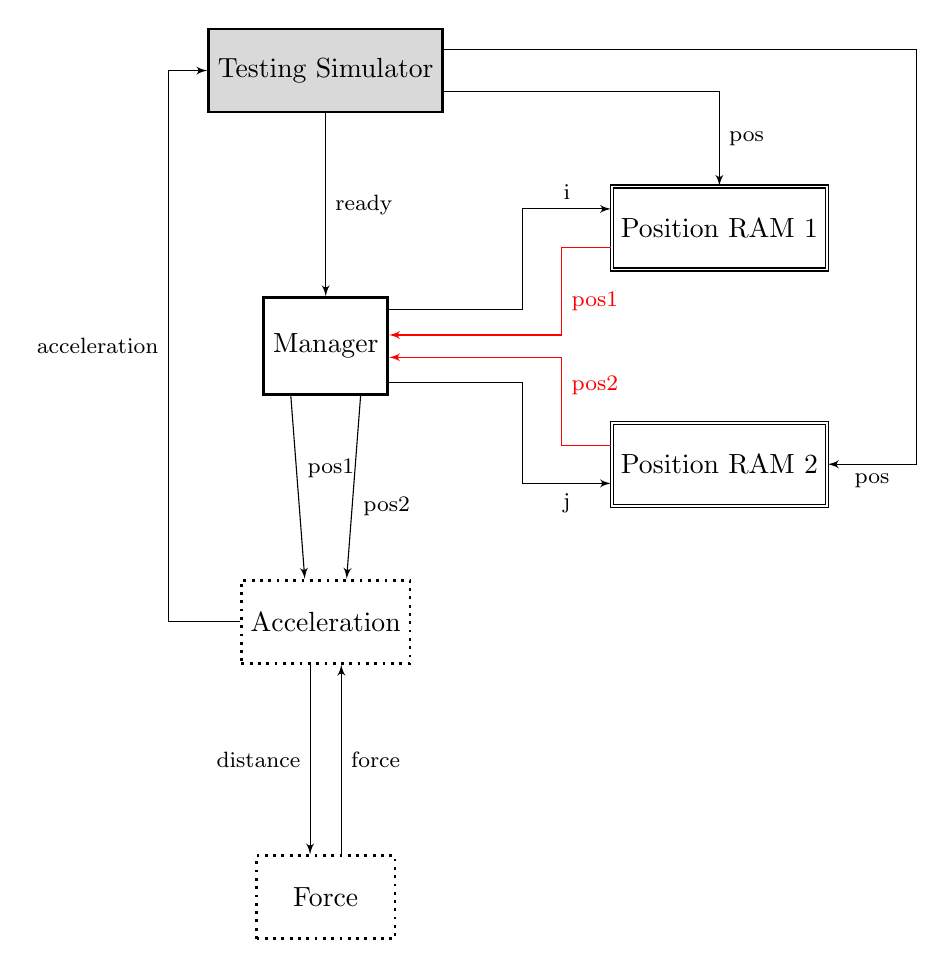
\begin{tikzpicture}
            \node[ram] (posram1) at (5,2) {Position RAM 1};
            \node[ram] (posram2) at (5,-1) {Position RAM 2};
            \node[process] (manager) at (0,.5) {Manager};
            \node[simulation] (testsim) at (0,4) {Testing Simulator};
            \node[module] (acceleration) at (0,-3) {Acceleration};
            \node[module] (force) at (0,-6.5) {Force};

            \path[draw, ->] (testsim.350) -| (posram1.90) node [near end] {\footnotesize pos};
            \path[draw, ->] (testsim.10) -| (7.5,-1) |- (posram2.0) node [near end] {\footnotesize pos};

            \path[draw, ->] (manager.30) -| (2.5,2) |- (posram1.170) node [near end] {\footnotesize i};
            \path[draw, ->] (manager.330) -| (2.5,0) |- (posram2.190) node [below,near end] {\footnotesize j};

            \path[draw, ->, red] (posram1.190) -| (3,1.5) |- (manager.10) node [near start] {\footnotesize pos1};
            \path[draw, ->, red] (posram2.170) -| (3,0) |- (manager.350) node [right,pos=0] {\footnotesize pos2};

            \path[draw, ->] (testsim.270) -- (manager.90) node [midway] {\footnotesize ready};

            \path[draw, ->] (manager.235) -- (acceleration.116) node [midway] {\footnotesize pos1};
            \path[draw, ->] (manager.305) -- (acceleration.64) node [midway] {\footnotesize pos2};

            \path[draw, ->] (acceleration.250) -- (force.110) node [midway, left] {\footnotesize distance};
            \path[draw, ->] (force.70) -- (acceleration.290) node [midway, right] {\footnotesize force};

            \path[draw, ->] (acceleration.180) -| (-2, -3) |- (testsim.180) node [near start] {\footnotesize acceleration};

        \end{tikzpicture}
    }
    \caption{Acceleration module 1.1}
\end{figure}

% -------------------------------------------------
% Acceleration 1.2

\begin{figure}
    \centering
    \scalebox{0.7}{
        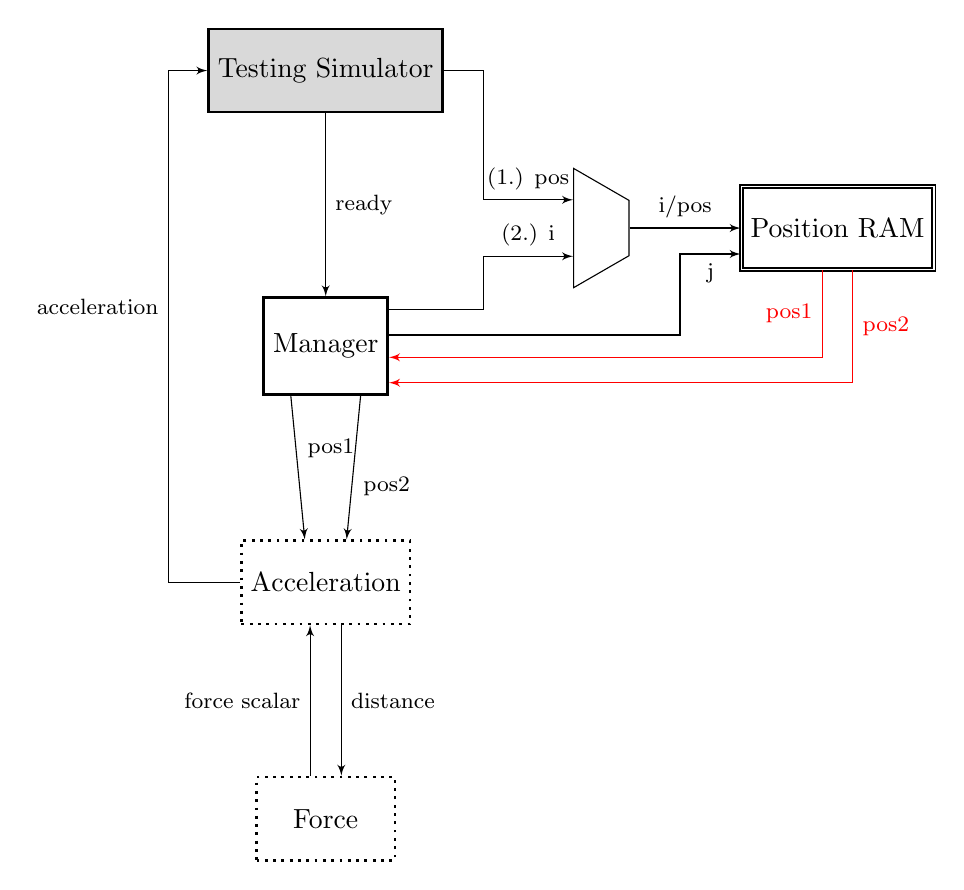
\begin{tikzpicture}
            \node[ram] (posram) at (6.5,1) {Position RAM};
            \node[multiplexer] (mux) at (3.5,1) {};
            \node[process] (manager) at (0,-.5) {Manager};
            \node[simulation] (testsim) at (0,3) {Testing Simulator};
            \node[module] (acceleration) at (0,-3.5) {Acceleration};
            \node[module] (force) at (0,-6.5) {Force};

            \path[draw, ->] (testsim.0) -| (2,3) |- (mux.north west) node [near end] {\footnotesize (1.) pos};
            \path[draw, ->] (manager.30) -| (2,0) |- (mux.south west) node [near end] {\footnotesize (2.) i};

            \path[draw, ->] (manager.10) -| (4.5,0) |- (posram.195) node [near end, below] {\footnotesize j};

            \path[draw, ->, red] (posram.250) |-  (manager.350) node [near start, left] {\footnotesize pos1};
            \path[draw, ->, red] (posram.290) |-  (manager.330) node [near start] {\footnotesize pos2};

            \path[draw, ->] (mux.top side) -- (posram.180) node [midway] {\footnotesize i/pos};


            \path[draw, ->] (testsim.270) -- (manager.90) node [midway] {\footnotesize ready};

            \path[draw, ->] (manager.235) -- (acceleration.116) node [midway] {\footnotesize pos1};
            \path[draw, ->] (manager.305) -- (acceleration.64) node [midway] {\footnotesize pos2};

            \path[draw, ->] (acceleration.290) -- (force.70) node [midway, right] {\footnotesize distance};
            \path[draw, ->] (force.110) -- (acceleration.250) node [midway, left] {\footnotesize force scalar};

            \path[draw, ->] (acceleration.180) -| (-2, -3) |- (testsim.180) node [near start] {\footnotesize acceleration};

        \end{tikzpicture}
    }
    \label{fig:acceleration-1-2}
    \caption{Acceleration module 1.2}
\end{figure}

% -------------------------------------------------
% Acceleration 1.3

%Acceleration module figure
\begin{figure}
    \centering
    \scalebox{0.7}{
        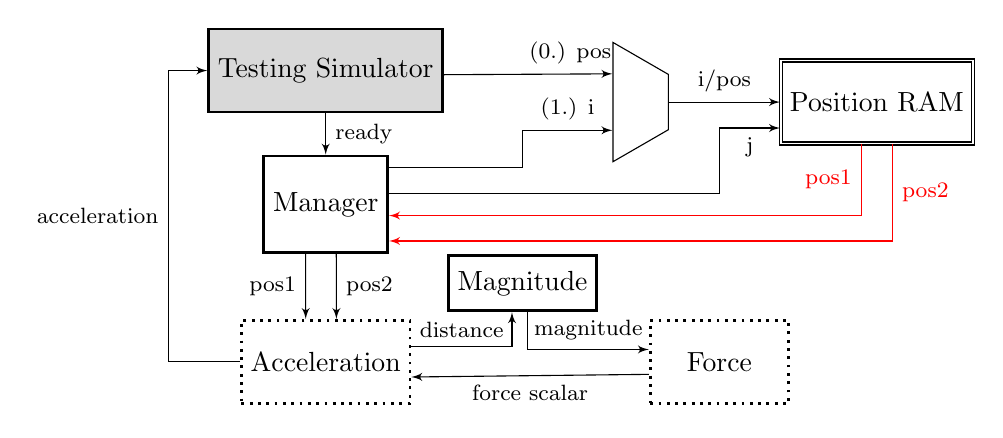
\begin{tikzpicture}
            \node[ram] (posram) at (6.5,0.8) {Position RAM};
            \node[multiplexer] (mux) at (3.5,0.8) {};
            \node[process] (manager) at (-0.5,-.5) {Manager};
            \node[simulation] (testsim) at (-0.5,1.2) {Testing Simulator};
            \node[module] (acceleration) at (-0.5,-2.5) {Acceleration};
            \node[module] (force) at (4.5,-2.5) {Force};
            \node[process, minimum height=2em] (mag) at (2,-1.5) {Magnitude};


            \path[draw, ->] (testsim.358) -- (mux.north west) node [near end] {\footnotesize (0.) pos};
            \path[draw, ->] (manager.30) -| (2,0) |- (mux.south west) node [near end] {\footnotesize (1.) i};

            \path[draw, ->] (manager.10) -| (4.5,0) |- (posram.195) node [near end, below] {\footnotesize j};

            \path[draw, ->, red] (posram.250) |-  (manager.350) node [near start, left] {\footnotesize pos1};
            \path[draw, ->, red] (posram.290) |-  (manager.330) node [near start] {\footnotesize pos2};

            \path[draw, ->] (mux.top side) -- (posram.180) node [midway] {\footnotesize i/pos};


            \path[draw, ->] (testsim.270) -- (manager.90) node [midway] {\footnotesize ready};

            \path[draw, ->] (manager.248) -- (acceleration.115) node [midway, left] {\footnotesize pos1};
            \path[draw, ->] (manager.282) -- (acceleration.76) node [midway] {\footnotesize pos2};

            \path[draw, ->] (acceleration.10) -| (mag.250) node [near start, above] {\footnotesize distance};
            \path[draw, ->] (mag.280) |- (force.170) node [near end, above] {\footnotesize magnitude};
            \path[draw, ->] (force.190) -- (acceleration.350) node [midway] {\footnotesize force scalar};

            \path[draw, ->] (acceleration.180) -| (-2.5, -2.5) |- (testsim.180) node [near start] {\footnotesize acceleration};

        \end{tikzpicture}
    }
    
    \caption{The complete design of the \texttt{Acceleration} module. The grayed out box represents \texttt{SimulationProcess}, the unfilled boxes represent \texttt{SimpleProcesses}, and double edge boxes represents RAM. The trapeze-shaped processes are multiplexor processes that choose between one bus or another, the numbering in the figure shows the priority order. The dotted squares represents a collection of \texttt{SimpleProcesses}, for instance \texttt{Force}. The internal structure of \texttt{Force} can be seen in Figure \ref{fig:force_depth}. The large blue dotted squares represent the different modules. The red lines represent the data being communicated from the RAM.}
    \label{fig:acceleration-1-3}
\end{figure}


% -------------------------------------------------
% Cache 1.1

\begin{figure}
    \centering
    \scalebox{0.8}{
        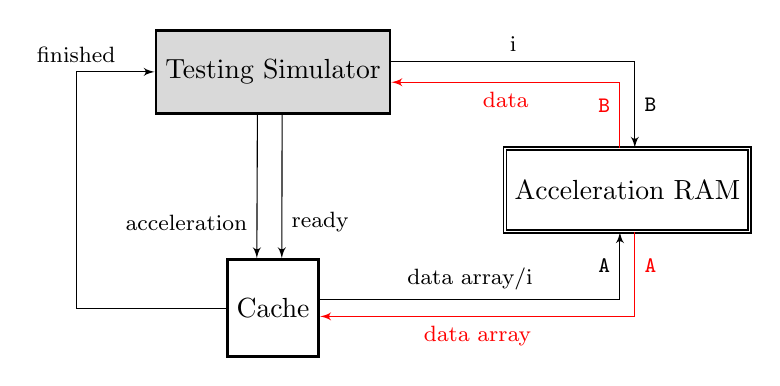
\begin{tikzpicture}
            \node[ram] (accram) at (4.5,-1.5) {Acceleration RAM};
            \node[simulation] (testsim) at (0,0) {Testing Simulator};
            \node[process] (cache) at (0,-3) {Cache};

            \path[draw, ->] (testsim.250) -- (cache.108) node [near end, left] {\footnotesize acceleration};
            \path[draw, ->] (testsim.282) -- (cache.80) node [near end] {\footnotesize ready};
            \path[draw, ->] (cache.10) -| node [near start] {\footnotesize data array/i} (accram.260) node [near end] {\footnotesize \texttt{A}};
            \path[draw, ->, red] (accram.280) |- node [pos=0.2] {\footnotesize \texttt{A}} (cache.350) node [near end] {\footnotesize data array};
            \path[draw, ->] (testsim.5) -| node [near start] {\footnotesize i} (accram.80) node [near end] {\footnotesize \texttt{B}};
            \path[draw, ->, red] (accram.100) |- node [pos=0.32] {\footnotesize \texttt{B}} (testsim.355) node [near end] {\footnotesize data};

            \path[draw, ->] (cache.180) -| (-2.5,-3) |- (testsim.180) node [midway] {\footnotesize finished};

        \end{tikzpicture}
    }
    \caption{Cache module 1.1}
\end{figure}

% -------------------------------------------------
% Velocity-(/position-)update module 1.1

\begin{figure}
    \centering
    \scalebox{0.8}{
        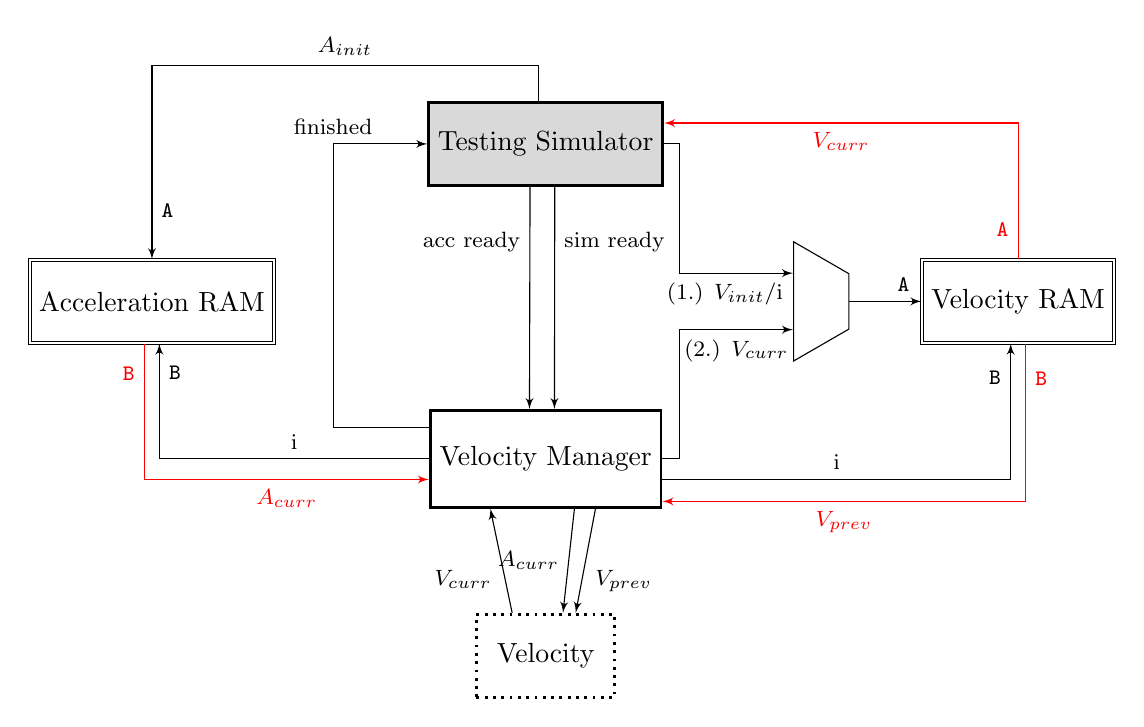
\begin{tikzpicture}
            \node[ram] (accram) at (-5,-2) {Acceleration RAM};
            \node[ram] (veloram) at (6,-2) {Velocity RAM};
            \node[simulation] (testsim) at (0,0) {Testing Simulator};
            \node[process] (manager) at (0,-4) {Velocity Manager};
            \node[module] (velocity) at (0,-6.5) {Velocity};
            \node[multiplexer, shape border rotate=270] (mux) at (3.5,-2) {};

            \path[draw, ->] (testsim.250) -- (manager.108) node [near start, left] {\footnotesize acc ready};
            \path[draw, ->] (testsim.282) -- (manager.80) node [near start] {\footnotesize sim ready};
            \path[draw, ->] (velocity.128) -- (manager.222) node [midway] {\footnotesize $V_{curr}$};
            \path[draw, ->] (manager.300) -- (velocity.68) node [midway, left] {\footnotesize $A_{curr}$};
            \path[draw, ->] (manager.315) -- (velocity.55) node [midway] {\footnotesize $V_{prev}$};

            \path[draw, ->] (manager.350) -| node [near start] {\footnotesize i} (veloram.260) node [very near end] {\footnotesize \texttt{B}};
            \path[draw, ->, red] (veloram.280) |- node [pos=0.11] {\footnotesize \texttt{B}} (manager.340) node [near end] {\footnotesize $V_{prev}$};

            \path[draw, ->] (manager.180) -| node [near start, above] {\footnotesize i} (accram.280) node [very near end, right] {\footnotesize \texttt{B}};
            \path[draw, ->, red] (accram.260) |- node [pos=0.11, left] {\footnotesize \texttt{B}} (manager.190) node [near end, below] {\footnotesize $A_{curr}$};
            \path[draw, ->] (manager.0) -| (1.7,-3) |- (mux.south west) node [near end, below] {\footnotesize (2.) $V_{curr}$};
            \path[draw, ->] (testsim.0) -| (1.7,-1) |- (mux.north west) node [pos=0.7, below] {\footnotesize (1.) $V_{init}$/i};

            \path[draw, ->] (mux.east) -- (veloram.180) node [near end] {\footnotesize \texttt{A}};
            \path[draw, ->] (testsim.100) |- (-5, 1) node [near end, above] {\footnotesize $A_{init}$} -| (accram.90) node [very near end] {\footnotesize \texttt{A}};

              \path[draw, ->, red] (veloram.90) |- node [pos=0.11] {\footnotesize \texttt{A}} (testsim.10) node [near end] {\footnotesize $V_{curr}$};

            \path[draw, ->] (manager.165) -| (-2.7,-3) |- (testsim.180) node [midway] {\footnotesize finished};

        \end{tikzpicture}
    }
    \caption{Velocity-(/Position)-update module 1.1}
\end{figure}


% -------------------------------------------------
% MD complete circuit

\begin{figure}
    \centering
    \scalebox{0.6}{
        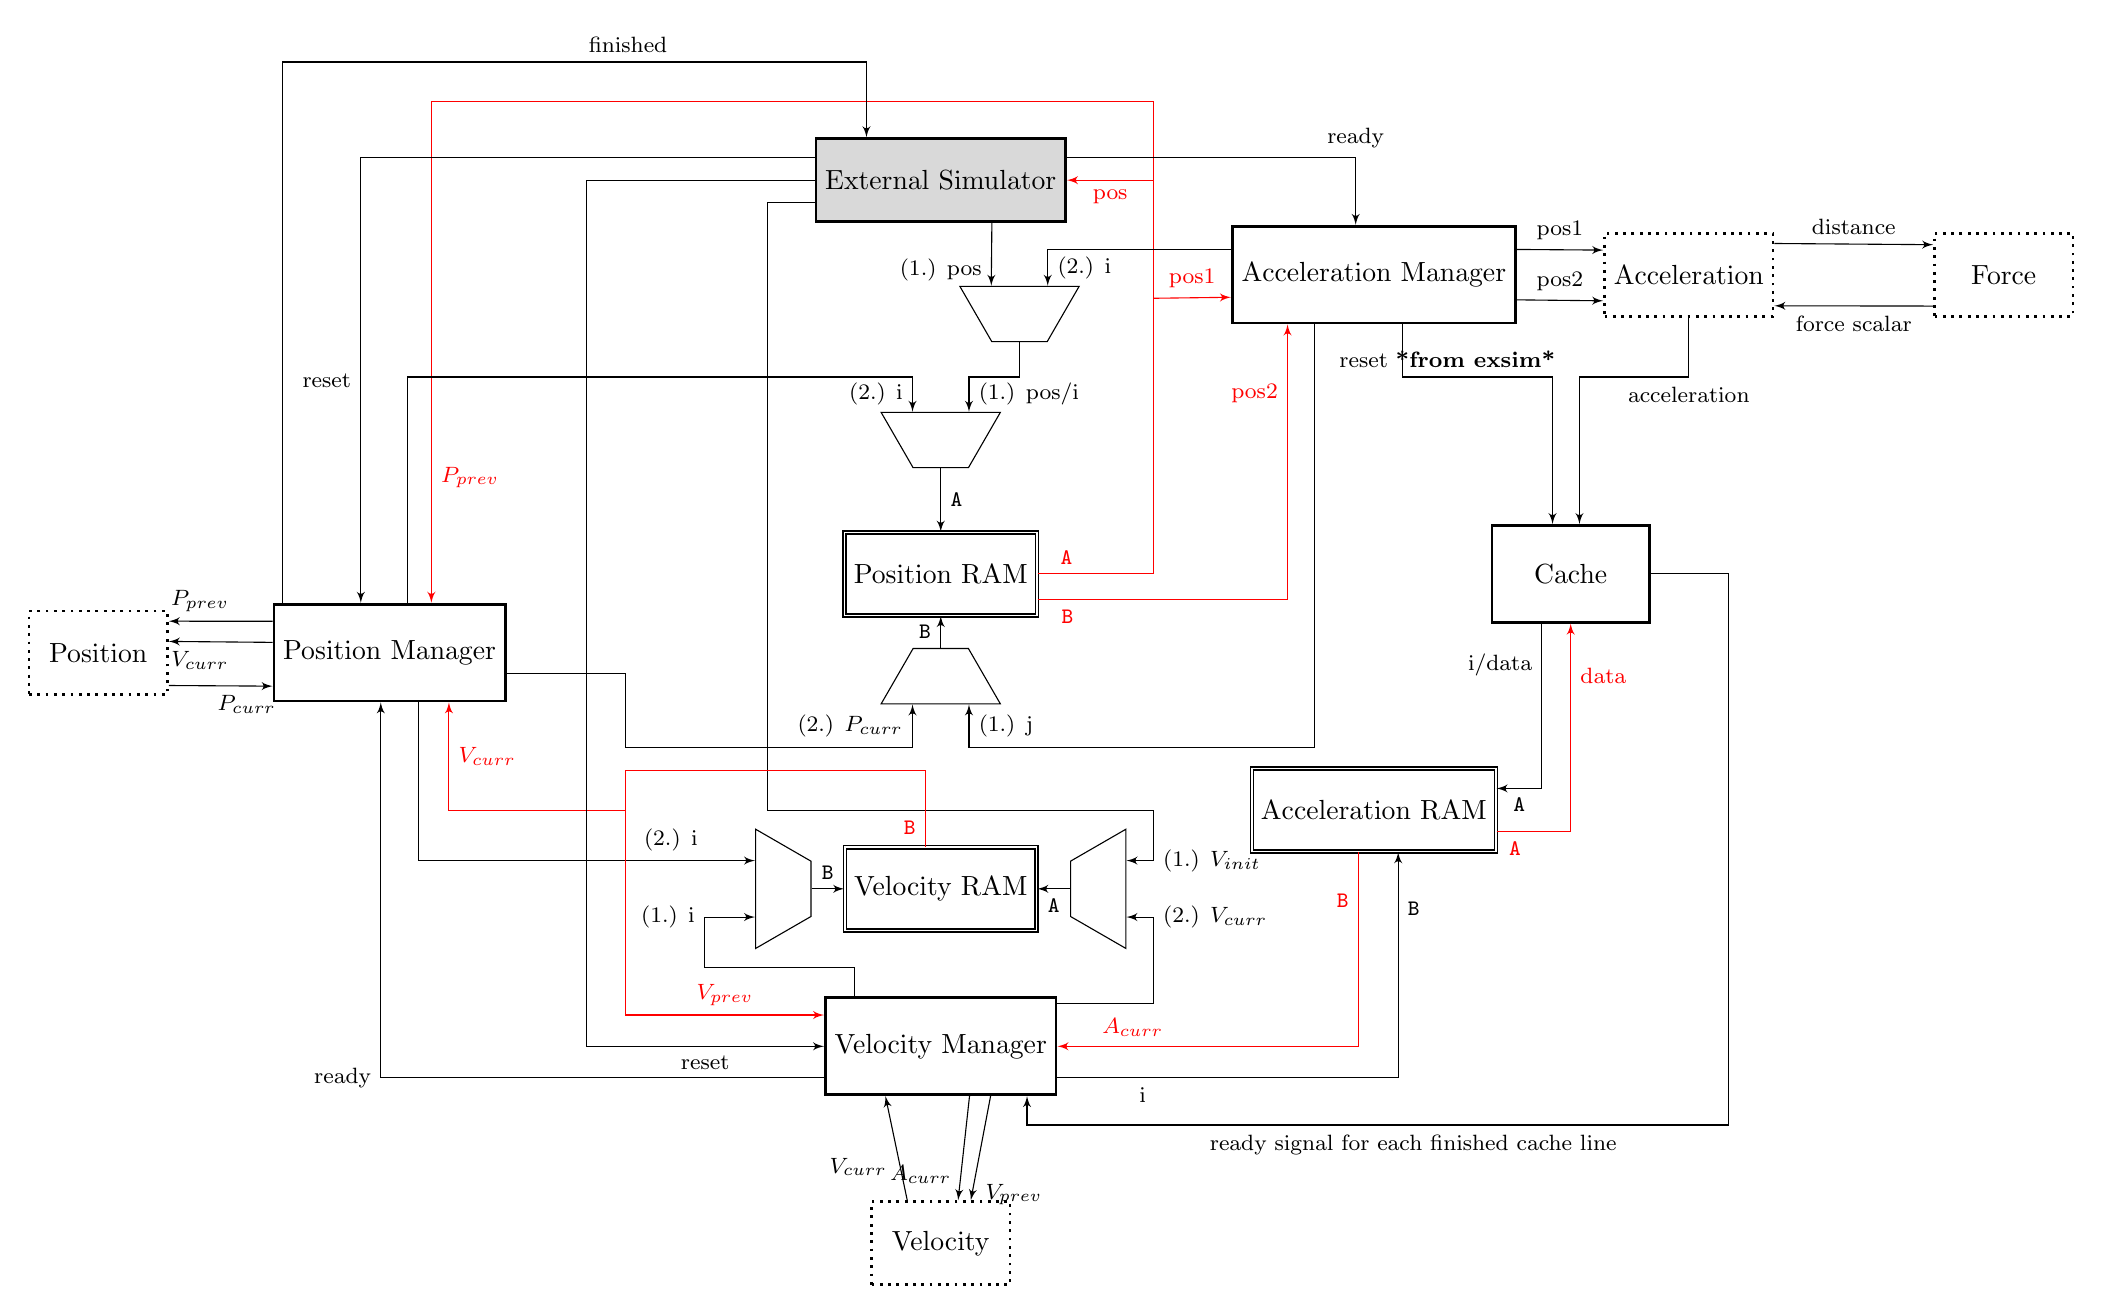
\begin{tikzpicture}
            \node[simulation] (exsim) at (0,0) {External Simulator};
            \node[ram] (posram) at (0,-5) {Position RAM};
            \node[ram] (accram) at (5.5,-8) {Acceleration RAM};
            \node[ram] (veloram) at (0,-9) {Velocity RAM};

            \node[multiplexer, shape border rotate=180] (mux1) at (1,-1.7) {};
            \node[multiplexer, shape border rotate=180] (mux2) at (0,-3.3) {};
            \node[multiplexer, shape border rotate=0] (mux3) at (0,-6.3) {};
            \node[multiplexer, shape border rotate=90] (mux4) at (2,-9) {};
            \node[multiplexer, shape border rotate=270] (mux5) at (-2,-9) {};
            \node[process] (accmanager) at (5.5,-1.2) {Acceleration Manager};
            \node[process, minimum width=2cm] (cache) at (8,-5) {Cache};
            \node[process] (velmanager) at (0,-11) {Velocity Manager};
            \node[process] (posmanager) at (-7,-6) {Position Manager};
            \node[module] (acceleration) at (9.5,-1.2) {Acceleration};
            \node[module] (force) at (13.5,-1.2) {Force};
            \node[module] (velocity) at (0,-13.5) {Velocity};
            \node[module] (position) at (-10.7,-6) {Position};

            \path[draw, ->] (exsim.320) -- (mux1.north west) node [left, near end] {\footnotesize (1.) pos};
            \path[draw, ->] (mux1.south) |- (1,-2.5) -| (mux2.north east) node [near end] {\footnotesize (1.) pos/i};
            \path[draw, ->] (mux2.south) -| (posram.90) node [near end] {\footnotesize \texttt{A}};


            \path[draw, ->, red] (posram.0) -| node [very near start] {\footnotesize \texttt{A}} (2.7,-5) |- (exsim.0) node [near end] {\footnotesize pos};

            \path[draw, ->, red] (2.7,-0) |- (2.7,1) -| (posmanager.50) node [very near end] {\footnotesize $P_{prev}$};
            \path[draw, ->, red] (2.7,-1.5) -- (accmanager.189) node [midway] {\footnotesize pos1};

            \path[draw, ->, red] (posram.345) -| node [pos=0.06, below] {\footnotesize \texttt{B}} (accmanager.210) node [very near end, left] {\footnotesize pos2};


            \path[draw, ->] (accmanager.170) -| (mux1.north east) node [near end] {\footnotesize (2.) i};
            \path[draw, ->] (accmanager.220) |- (4.5,-7.2) -| (mux3.south east) node [near end, right] {\footnotesize (1.) j};

            \path[draw, ->] (exsim.10) -| (accmanager.110) node [midway, above] {\footnotesize ready};

            \path[draw, ->] (accmanager.300) |- (7,-2.5) node [near end] {\footnotesize reset \textbf{*from exsim*}} -| (cache.110) ;

            \path[draw, ->] (acceleration.270) |- node [midway] {\footnotesize acceleration} (9,-2.5) -| (cache.80) ;

            \path[draw, ->] (cache.240) |- node [very near start, left] {\footnotesize i/data} (accram.10) node [near end] {\footnotesize \texttt{A}};
            \path[draw, ->, red] (accram.350) -| node [very near start, below] {\footnotesize \texttt{A}} (cache.270) node [very near end, right] {\footnotesize data};

            \path[draw, ->] (accmanager.10) -- (acceleration.164) node [midway] {\footnotesize pos1};
            \path[draw, ->] (accmanager.350) -- (acceleration.197) node [midway] {\footnotesize pos2};

            \path[draw, ->] (acceleration.20) -- (force.157) node [midway] {\footnotesize distance};
            \path[draw, ->] (force.204) -- (acceleration.340) node [midway] {\footnotesize force scalar};

            \path[draw, ->, red] (accram.250) |- node [very near start, left] {\footnotesize \texttt{B}} (velmanager.0) node [very near end, above] {\footnotesize $A_{curr}$};
            \path[draw, ->] (velmanager.345) -| node [very near start, below] {\footnotesize i} (accram.300) node [very near end, right] {\footnotesize \texttt{B}};

            \path[draw, ->] (cache.0) -| (10, -5) |- node [near end] {\footnotesize ready signal for each finished cache line} (2,-12) -| (velmanager.330);

            \path[draw, ->] (velmanager.300) -- (velocity.68) node [near end, left] {\footnotesize $A_{curr}$};
            \path[draw, ->] (velmanager.315) -- (velocity.55) node [near end] {\footnotesize $V_{prev}$};
            \path[draw, ->] (velocity.128) -- (velmanager.222) node [midway] {\footnotesize $V_{curr}$};


            \path[draw, ->] (mux4.west) -- (veloram.0) node [midway] {\footnotesize \texttt{A}};

            \path[draw, ->] (velmanager.20) -| (2.7,-10) |- node [midway, right] {\footnotesize (2.) $V_{curr}$} (mux4.south east);
            \path[draw, ->] (exsim.190) -| (-2.2,-8) -| (2.7,-8) |- node [midway, right] {\footnotesize (1.) $V_{init}$} (mux4.north east);

            \path[draw, ->] (mux5.east) -- (veloram.180) node [midway] {\footnotesize \texttt{B}};

            \path[draw, ->] (velmanager.150) |- (-3,-10) |- node [midway, left] {\footnotesize (1.) i} (mux5.south west);
            \path[draw, ->] (posmanager.300) |- node [very near end] {\footnotesize (2.) i} (mux5.north west);

            \path[draw, ->, red] (veloram.110) |- node [very near start] {\footnotesize \texttt{B}} (-3, -7.5) -| (-4,-8) |- (velmanager.165) node [near end] {\footnotesize $V_{prev}$};

            \path[draw, ->, red] (-4,-8) -| (posmanager.320) node [near end, right] {\footnotesize $V_{curr}$};

            \path[draw, ->] (exsim.180) -| (-4.5,-11) |- (velmanager.180) node [near end, below] {\footnotesize reset};

            \path[draw, ->] (posmanager.165) -- (position.24) node [pos=0.7, above] {\footnotesize $P_{prev}$};
            \path[draw, ->] (posmanager.175) -- (position.9) node [pos=0.7] {\footnotesize $V_{curr}$};
            \path[draw, ->] (position.335) -- (posmanager.196) node [near end, below] {\footnotesize $P_{curr}$};

            \path[draw, ->] (velmanager.195) -| (posmanager.260) node [midway] {\footnotesize ready};


            \path[draw, ->] (mux3.north) -- (posram.270) node [midway] {\footnotesize \texttt{B}};

            \path[draw, ->] (posmanager.350) -| (-4,-6.5) |- (-4,-7.2) -| (mux3.south west) node [near end, left] {\footnotesize (2.) $P_{curr}$};

            \path[draw, ->] (posmanager.70) |- (-4,-2.5) -| (mux2.north west) node [near end, left] {\footnotesize (2.) i};

            \path[draw, ->] (exsim.170) -| (posmanager.120) node [near end, left] {\footnotesize reset};

            \path[draw, ->] (posmanager.155) |- (-7,1.5) -| node [near start] {\footnotesize finished} (exsim.150) ;
        \end{tikzpicture}
    }
    \caption{Full MD circuit}
\end{figure}


%-----------------
% Full circuit 2.0

% Full circuit figure
\begin{figure*}
    \centering
    \scalebox{0.6}{
        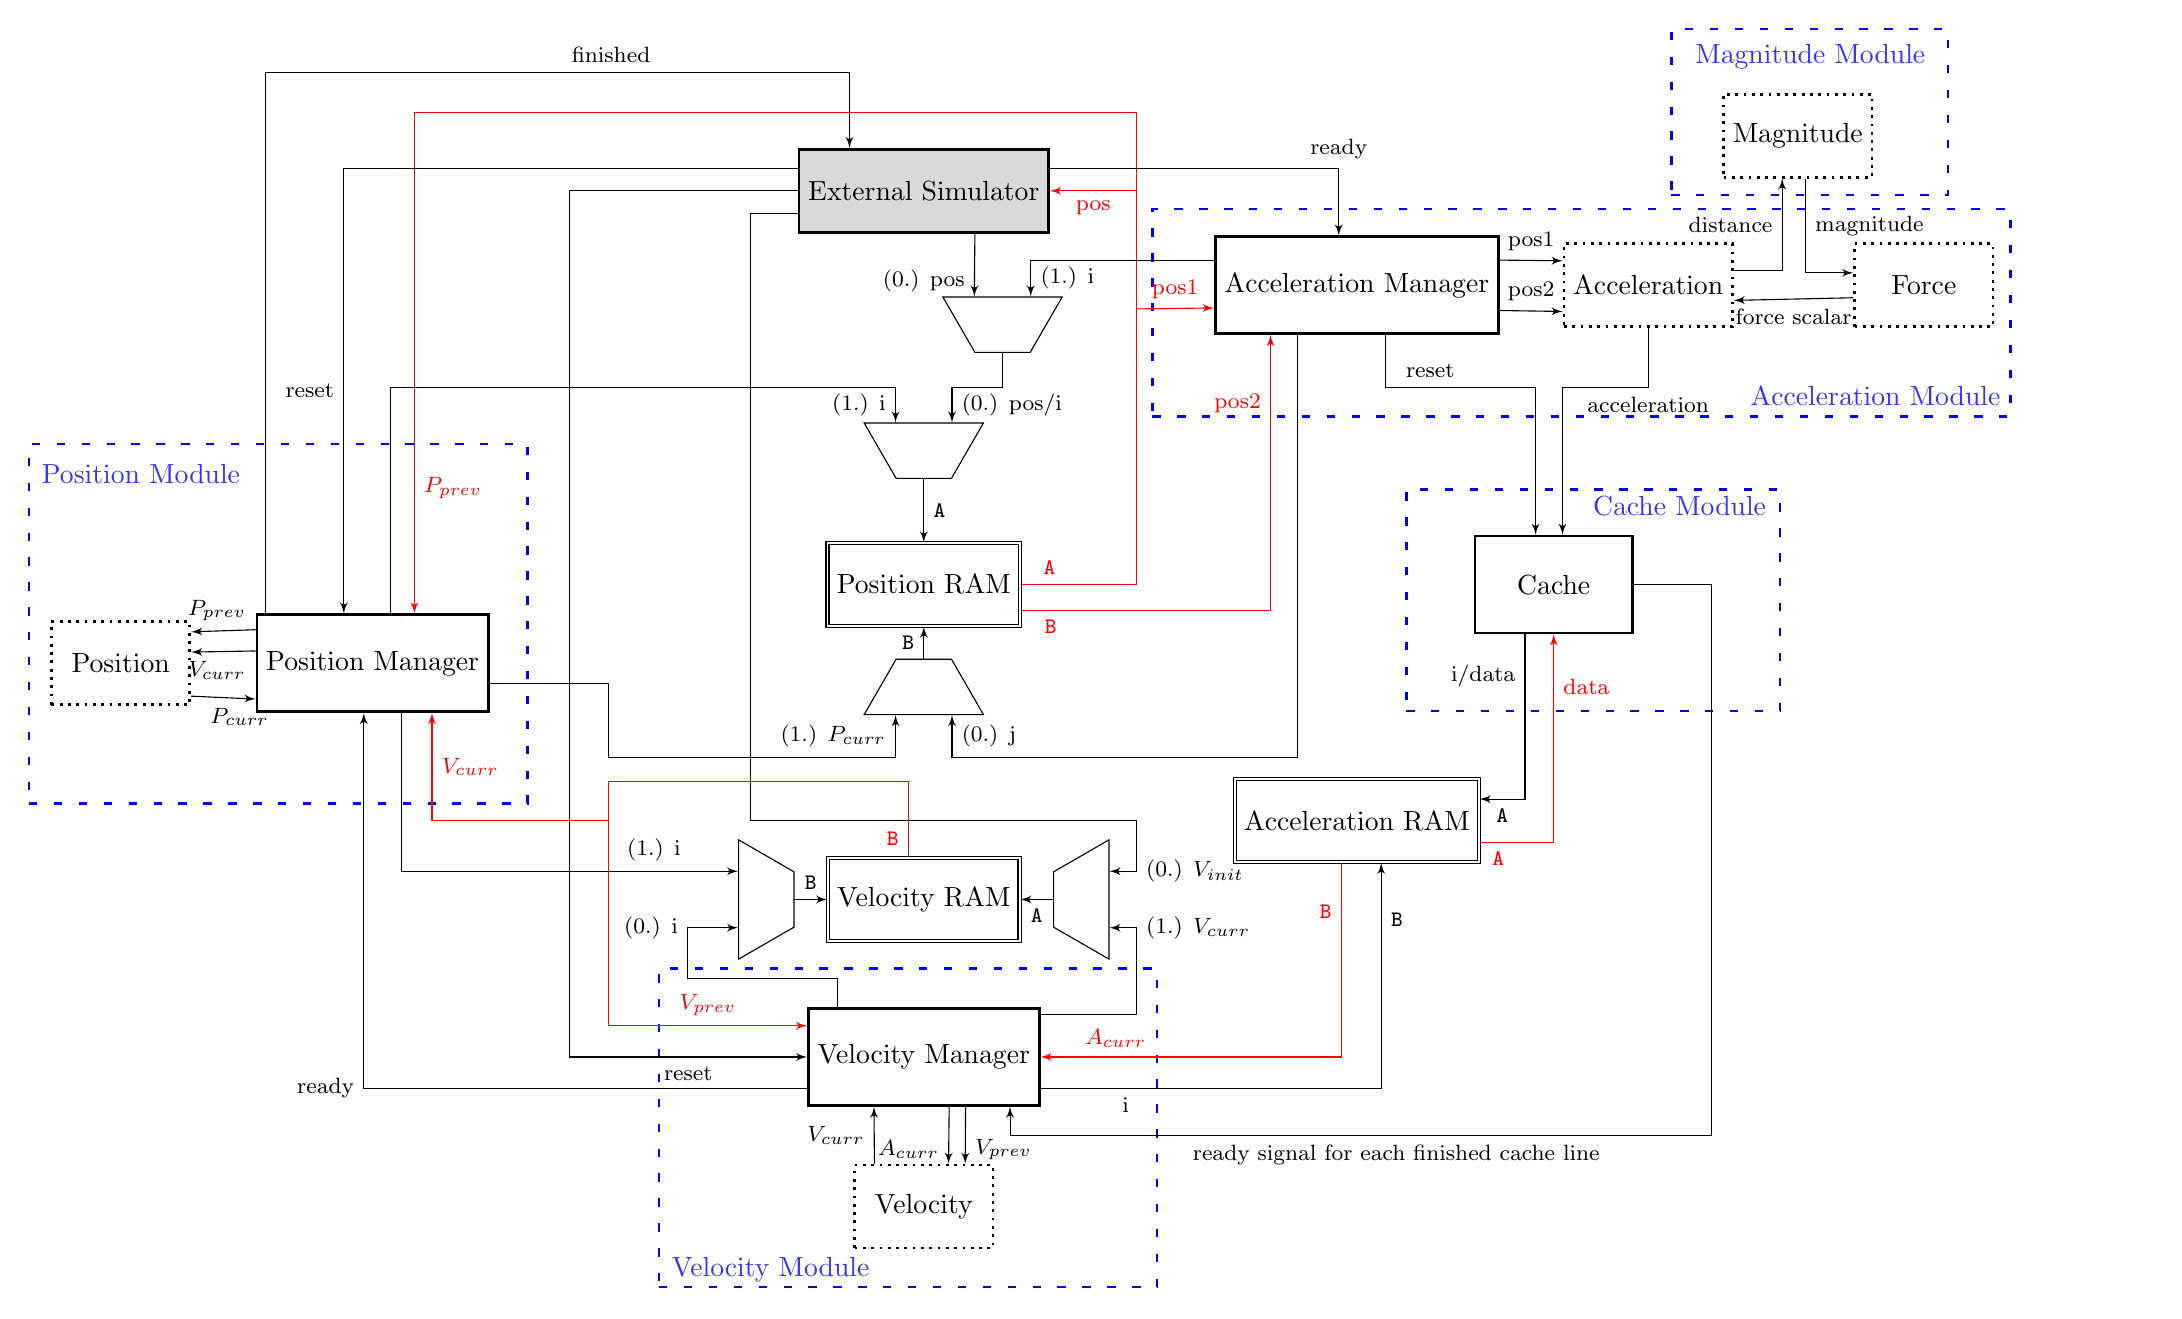
\begin{tikzpicture}
            \node[simulation] (exsim) at (0,0) {External Simulator};
            \node[ram] (posram) at (0,-5) {Position RAM};
            \node[ram] (accram) at (5.5,-8) {Acceleration RAM};
            \node[ram] (veloram) at (0,-9) {Velocity RAM};

            \node[multiplexer, shape border rotate=180] (mux1) at (1,-1.7) {};
            \node[multiplexer, shape border rotate=180] (mux2) at (0,-3.3) {};
            \node[multiplexer, shape border rotate=0] (mux3) at (0,-6.3) {};
            \node[multiplexer, shape border rotate=90] (mux4) at (2,-9) {};
            \node[multiplexer, shape border rotate=270] (mux5) at (-2,-9) {};
            \node[process] (accmanager) at (5.5,-1.2) {Acceleration Manager};
            \node[process, minimum width=2cm] (cache) at (8,-5) {Cache};
            \node[process] (velmanager) at (0,-11) {Velocity Manager};
            \node[process] (posmanager) at (-7,-6) {Position Manager};
            \node[module] (acceleration) at (9.2,-1.2) {Acceleration};
            \node[module] (force) at (12.7,-1.2) {Force};
            \node[module, minimum height=3em, align=center] (mag) at (11.1,0.7) {Magnitude};
            \node[module] (velocity) at (0,-12.9) {Velocity};
            \node[module] (position) at (-10.2,-6) {Position};

            %Acceleration module
            \node[toplevel, minimum height=7.5em, minimum width=31em] (accmodule) at (8.35,-1.55) {};
            \node[text width=5cm, blue!80] at (13,-2.6) {Acceleration Module};
            
            % Magnitude module
            \node[toplevel, minimum height=6em, minimum width=10em] (magmodule) at (11.25,1) {};
            \node[text width=5cm, blue!80] at (12.3,1.7) {Magnitude Module};

            % Cache module
            \node[toplevel, minimum height=8em, minimum width=13.5em] (cachemodule) at (8.5,-5.2) {};
            \node[text width=5cm, blue!80] at (11,-4) {Cache Module};

            % Velocity module
            \node[toplevel, minimum height=11.5em, minimum width=18em] (velmodule) at (-.2,-11.9) {};
            \node[text width=5cm, blue!80] at (-0.7,-13.7) {Velocity Module};

            % Position module
            \node[toplevel, minimum height=13em, minimum width=18em] (posmodule) at (-8.2,-5.5) {};
            \node[text width=5cm, blue!80] at (-8.7,-3.6) {Position Module};
            
            
            \path[draw, ->] (exsim.320) -- (mux1.north west) node [left, near end] {\footnotesize (0.) pos};
            \path[draw, ->] (mux1.south) |- (1,-2.5) -| (mux2.north east) node [near end] {\footnotesize (0.) pos/i};
            \path[draw, ->] (mux2.south) -| (posram.90) node [near end] {\footnotesize \texttt{A}};


            \path[draw, ->, red] (posram.0) -| node [very near start] {\footnotesize \texttt{A}} (2.7,-5) |- (exsim.0) node [near end] {\footnotesize pos};

            \path[draw, ->, red] (2.7,-0) |- (2.7,1) -| (posmanager.50) node [very near end] {\footnotesize $P_{prev}$};
            \path[draw, ->, red] (2.7,-1.5) -- (accmanager.189) node [midway] {\footnotesize pos1};

            \path[draw, ->, red] (posram.345) -| node [pos=0.06, below] {\footnotesize \texttt{B}} (accmanager.210) node [very near end, left] {\footnotesize pos2};


            \path[draw, ->] (accmanager.170) -| (mux1.north east) node [near end] {\footnotesize (1.) i};
            \path[draw, ->] (accmanager.220) |- (4.5,-7.2) -| (mux3.south east) node [near end, right] {\footnotesize (0.) j};

            \path[draw, ->] (exsim.10) -| (accmanager.110) node [midway, above] {\footnotesize ready};

            \path[draw, ->] (accmanager.300) |- (7,-2.5) node [near end] {\footnotesize reset} -| (cache.110) ;

            \path[draw, ->] (acceleration.270) |- node [midway] {\footnotesize acceleration} (9,-2.5) -| (cache.80) ;

            \path[draw, ->] (cache.240) |- node [very near start, left] {\footnotesize i/data} (accram.10) node [near end] {\footnotesize \texttt{A}};
            \path[draw, ->, red] (accram.350) -| node [very near start, below] {\footnotesize \texttt{A}} (cache.270) node [very near end, right] {\footnotesize data};

            \path[draw, ->] (accmanager.10) -- (acceleration.164) node [midway] {\footnotesize pos1};
            \path[draw, ->] (accmanager.350) -- (acceleration.197) node [midway] {\footnotesize pos2};

            \path[draw, ->] (acceleration.10) -| (mag.250) node [near end, left] {\footnotesize distance};
            \path[draw, ->] (mag.280) |- (force.170) node [near start, right] {\footnotesize magnitude};
            \path[draw, ->] (force.190) -- (acceleration.350) node [midway] {\footnotesize force scalar};

            \path[draw, ->, red] (accram.250) |- node [very near start, left] {\footnotesize \texttt{B}} (velmanager.0) node [very near end, above] {\footnotesize $A_{curr}$};
            \path[draw, ->] (velmanager.345) -| node [very near start, below] {\footnotesize i} (accram.300) node [very near end, right] {\footnotesize \texttt{B}};

            \path[draw, ->] (cache.0) -| (10, -5) |- node [near end] {\footnotesize ready signal for each finished cache line} (2,-12) -| (velmanager.330);

            \path[draw, ->] (velmanager.297) -- (velocity.60) node [near end, left] {\footnotesize $A_{curr}$};
            \path[draw, ->] (velmanager.310) -- (velocity.46) node [near end] {\footnotesize $V_{prev}$};
            \path[draw, ->] (velocity.139) -- (velmanager.225) node [midway] {\footnotesize $V_{curr}$};


            \path[draw, ->] (mux4.west) -- (veloram.0) node [midway] {\footnotesize \texttt{A}};

            \path[draw, ->] (velmanager.20) -| (2.7,-10) |- node [midway, right] {\footnotesize (1.) $V_{curr}$} (mux4.south east);
            \path[draw, ->] (exsim.190) -| (-2.2,-8) -| (2.7,-8) |- node [midway, right] {\footnotesize (0.) $V_{init}$} (mux4.north east);

            \path[draw, ->] (mux5.east) -- (veloram.180) node [midway] {\footnotesize \texttt{B}};

            \path[draw, ->] (velmanager.150) |- (-3,-10) |- node [midway, left] {\footnotesize (0.) i} (mux5.south west);
            \path[draw, ->] (posmanager.300) |- node [very near end] {\footnotesize (1.) i} (mux5.north west);

            \path[draw, ->, red] (veloram.110) |- node [very near start] {\footnotesize \texttt{B}} (-3, -7.5) -| (-4,-8) |- (velmanager.165) node [near end] {\footnotesize $V_{prev}$};

            \path[draw, ->, red] (-4,-8) -| (posmanager.320) node [near end, right] {\footnotesize $V_{curr}$};

            \path[draw, ->] (exsim.180) -| (-4.5,-11) |- (velmanager.180) node [near end, below] {\footnotesize reset};

            \path[draw, ->] (posmanager.164) -- (position.24) node [pos=0.6, above] {\footnotesize $P_{prev}$};
            \path[draw, ->] (posmanager.174) -- (position.9) node [pos=0.6] {\footnotesize $V_{curr}$};
            \path[draw, ->] (position.335) -- (posmanager.197) node [near end, below] {\footnotesize $P_{curr}$};

            \path[draw, ->] (velmanager.195) -| (posmanager.260) node [midway] {\footnotesize ready};


            \path[draw, ->] (mux3.north) -- (posram.270) node [midway] {\footnotesize \texttt{B}};

            \path[draw, ->] (posmanager.350) -| (-4,-6.5) |- (-4,-7.2) -| (mux3.south west) node [near end, left] {\footnotesize (1.) $P_{curr}$};

            \path[draw, ->] (posmanager.70) |- (-4,-2.5) -| (mux2.north west) node [near end, left] {\footnotesize (1.) i};

            \path[draw, ->] (exsim.170) -| (posmanager.120) node [near end, left] {\footnotesize reset};

            \path[draw, ->] (posmanager.155) |- (-7,1.5) -| node [near start] {\footnotesize finished} (exsim.150) ;
        \end{tikzpicture}
    }
    \caption{The entire MD simulation network. Each box represents a process. The grayed out box represents \texttt{SimulationProcess}, the unfilled boxes represent \texttt{SimpleProcesses}, and double edge boxes represents RAM. The trapeze-shaped processes are multiplexor processes that choose between one bus or another, the numbering in the figure shows the priority order. The dotted squares represents a collection of \texttt{SimpleProcesses}, for instance \texttt{Force}. The internal structure of \texttt{Force} can be seen in Figure \ref{fig:force_depth}. The large blue dotted squares represent the different modules. The red lines represent the data being communicated from the RAM.}
    \label{fig:full_circuit}
\end{figure*}

% -------------------------------------------------
% Cache 1.1


\section{Function wrappers}
Force: $$f = \left(48 \cdot \epsilon \cdot \left( \frac{\sigma^{12}}{r^{14}}\right)\right) - \left(24 \cdot \epsilon \cdot\left(\frac{\sigma^6}{r^8} \right) \right)$$
Acceleration:
$$
r = x1 - x2
mag = \sqrt{r^2}
f_scalar = force(mag)
f = f_scalar * r
accel = f / mass
$$


\begin{figure}
    \centering
    \scalebox{0.8}{
        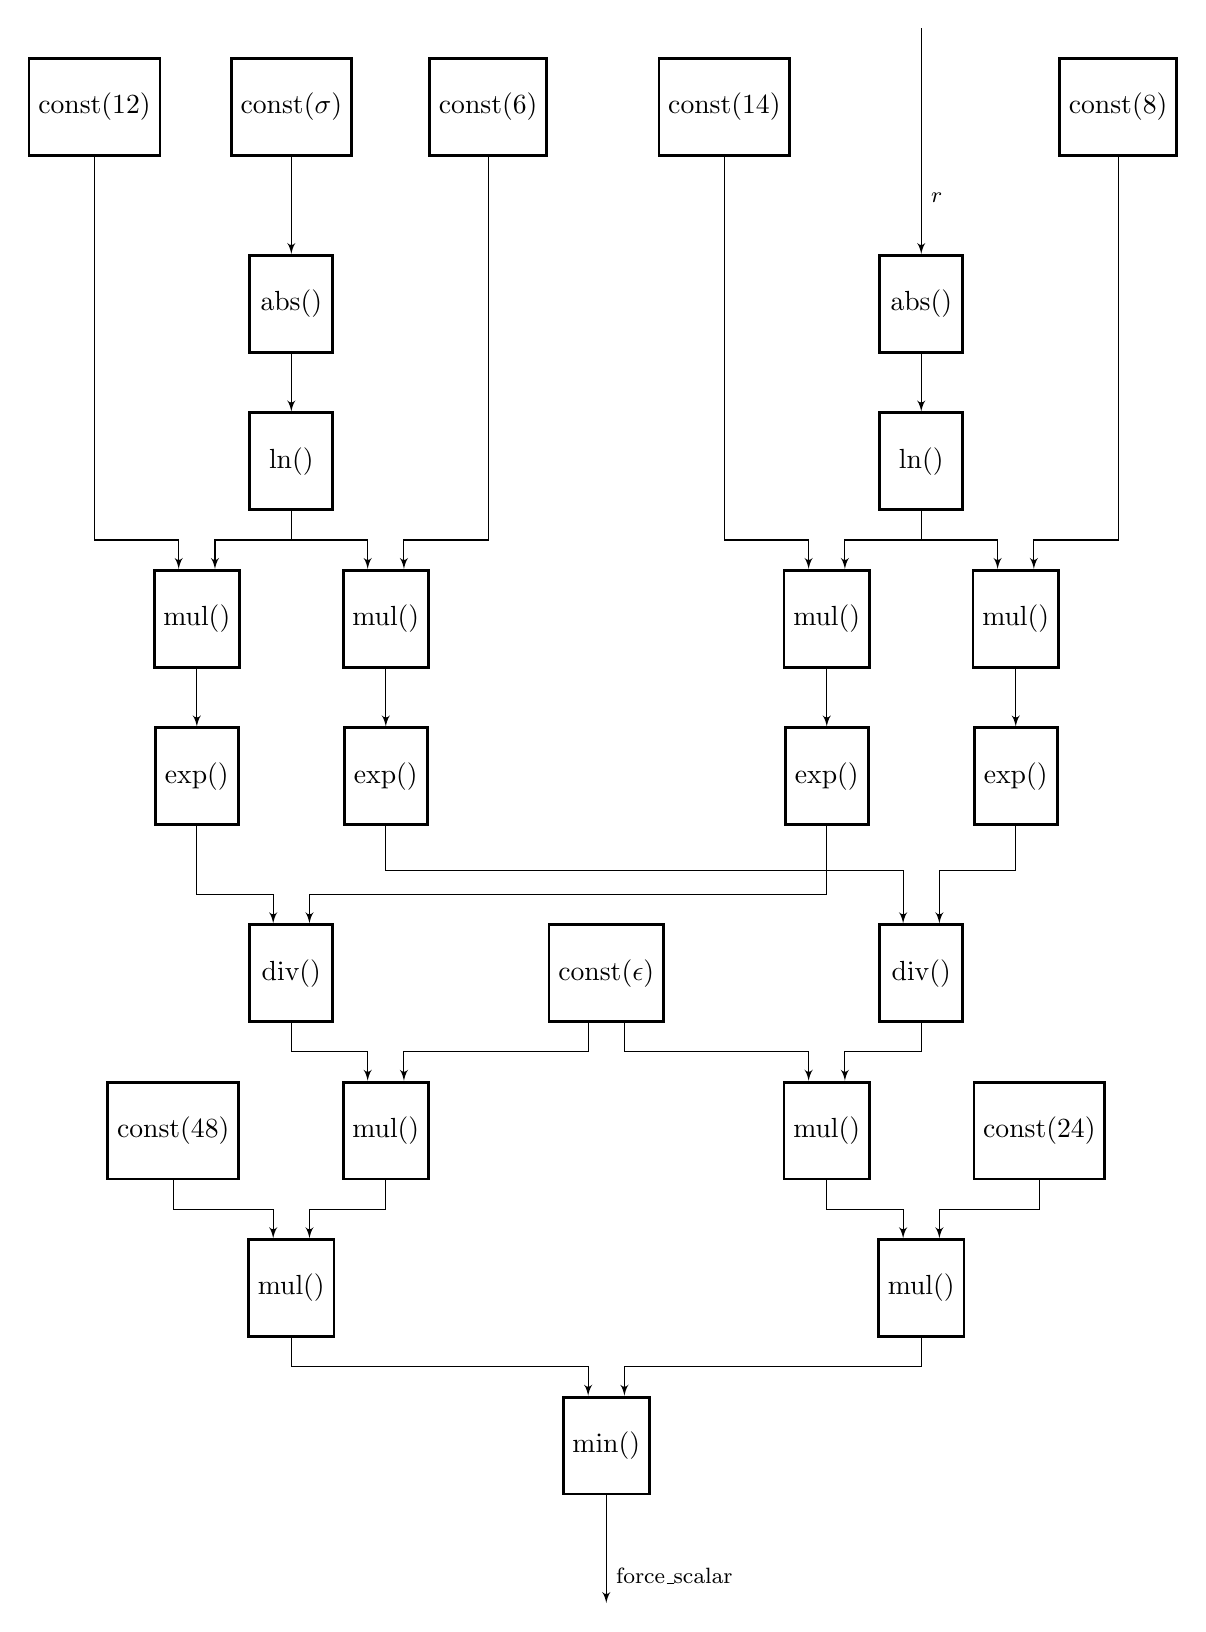
\begin{tikzpicture}

            \node[process] (twelve) at (-6.5,0) {const(12)};
            \node[process] (six) at (-1.5,0) {const(6)};
            \node[process] (sigma) at (-4,0) {const($\sigma$)};
            \node[process] (abs_sigma) at (-4,-2.5) {abs()};
            \node[process] (ln_sigma) at (-4,-4.5) {ln()};

            \node[process] (fourteen) at (1.5,0) {const(14)};
            \node[process] (eight) at (6.5,0) {const(8)};
            \node[process] (abs_r) at (4,-2.5) {abs()};
            \node[process] (ln_r) at (4,-4.5) {ln()};

            
            \node[process] (mul_12) at (-5.2,-6.5) {mul()};
            \node[process] (mul_6) at (-2.8,-6.5) {mul()};

            \node[process] (mul_14) at (2.8,-6.5) {mul()};
            \node[process] (mul_8) at (5.2,-6.5) {mul()};

            \node[process] (exp_12) at (-5.2,-8.5) {exp()};
            \node[process] (exp_6) at (-2.8,-8.5) {exp()};

            \node[process] (exp_14) at (2.8,-8.5) {exp()};
            \node[process] (exp_8) at (5.2,-8.5) {exp()};
            
            \node[process] (div_12_14) at (-4,-11) {div()};
            \node[process] (div_6_8) at (4,-11) {div()};

            \node[process] (epsilon) at (0,-11) {const($\epsilon$)};

            \node[process] (mul_12_14_eps) at (-2.8,-13) {mul()};
            \node[process] (mul_6_8_eps) at (2.8,-13) {mul()};

            \node[process] (fortyeight) at (-5.5,-13) {const(48)};
            \node[process] (twentyfour) at (5.5,-13) {const(24)};

            \node[process] (mul_48) at (-4,-15) {mul()};
            \node[process] (mul_24) at (4,-15) {mul()};

            \node[process] (min) at (0,-17) {min()};
            

            \path[draw, ->] (sigma.270) -- (abs_sigma.90);
            \path[draw, ->] (4,1) -- (abs_r.90) node [near end] {\footnotesize $r$};

            \path[draw, ->] (abs_sigma.270) -- (ln_sigma.90);
            \path[draw, ->] (abs_r.270) -- (ln_r.90);


            \path[draw, ->] (twelve.270) |- (-5.5, -5.5) -| (mul_12.110);
            \path[draw, ->] (ln_sigma.270) |- (-4.5, -5.5) -| (mul_12.70);
            
            \path[draw, ->] (six.270) |- (-2, -5.5) -| (mul_6.70);
            \path[draw, ->] (ln_sigma.270) |- (-3.5, -5.5) -| (mul_6.110);

            \path[draw, ->] (fourteen.270) |- (2, -5.5) -| (mul_14.110);
            \path[draw, ->] (ln_r.270) |- (3.5, -5.5) -| (mul_14.70);
            
            \path[draw, ->] (eight.270) |- (5.5, -5.5) -| (mul_8.70);
            \path[draw, ->] (ln_r.270) |- (4.5, -5.5) -| (mul_8.110);

            \path[draw, ->] (mul_12.270) -- (exp_12.90);
            \path[draw, ->] (mul_6.270) -- (exp_6.90);

            \path[draw, ->] (mul_14.270) -- (exp_14.90);
            \path[draw, ->] (mul_8.270) -- (exp_8.90);

            \path[draw, ->] (exp_12.270) |- (-4.5, -10) -| (div_12_14.110);
            \path[draw, ->] (exp_14.270) |- (-3.5, -10) -| (div_12_14.70);

            \path[draw, ->] (exp_6.270) |- (3.5, -9.7) -| (div_6_8.110);
            \path[draw, ->] (exp_8.270) |- (4.5, -9.7) -| (div_6_8.70);

            \path[draw, ->] (div_12_14.270) |- (-3.5, -12) -| (mul_12_14_eps.110);
            \path[draw, ->] (epsilon.250) |- (-2.5, -12) -| (mul_12_14_eps.70);
            
            \path[draw, ->] (div_6_8.270) |- (3.5, -12) -| (mul_6_8_eps.70);
            \path[draw, ->] (epsilon.290) |- (2.5, -12) -| (mul_6_8_eps.110);

            \path[draw, ->] (fortyeight.270) |- (-4.5, -14) -| (mul_48.110);
            \path[draw, ->] (mul_12_14_eps.270) |- (-3.5, -14) -| (mul_48.70);

            \path[draw, ->] (twentyfour.270) |- (4.5, -14) -| (mul_24.70);
            \path[draw, ->] (mul_6_8_eps.270) |- (3.5, -14) -| (mul_24.110);

            \path[draw, ->] (mul_48.270) |- (-3.5, -16) -| (min.110);
            \path[draw, ->] (mul_24.270) |- (2.5, -16) -| (min.70);

            \path[draw, ->] (min.270) -- (0,-19) node [near end] {\footnotesize force\_scalar};

        \end{tikzpicture}
        }
    \caption{Force wrapper}
\end{figure}


%-----------
% Force depth 2.0
%Force depth figure
\begin{figure*}
    \centering
    \scalebox{0.65}{
        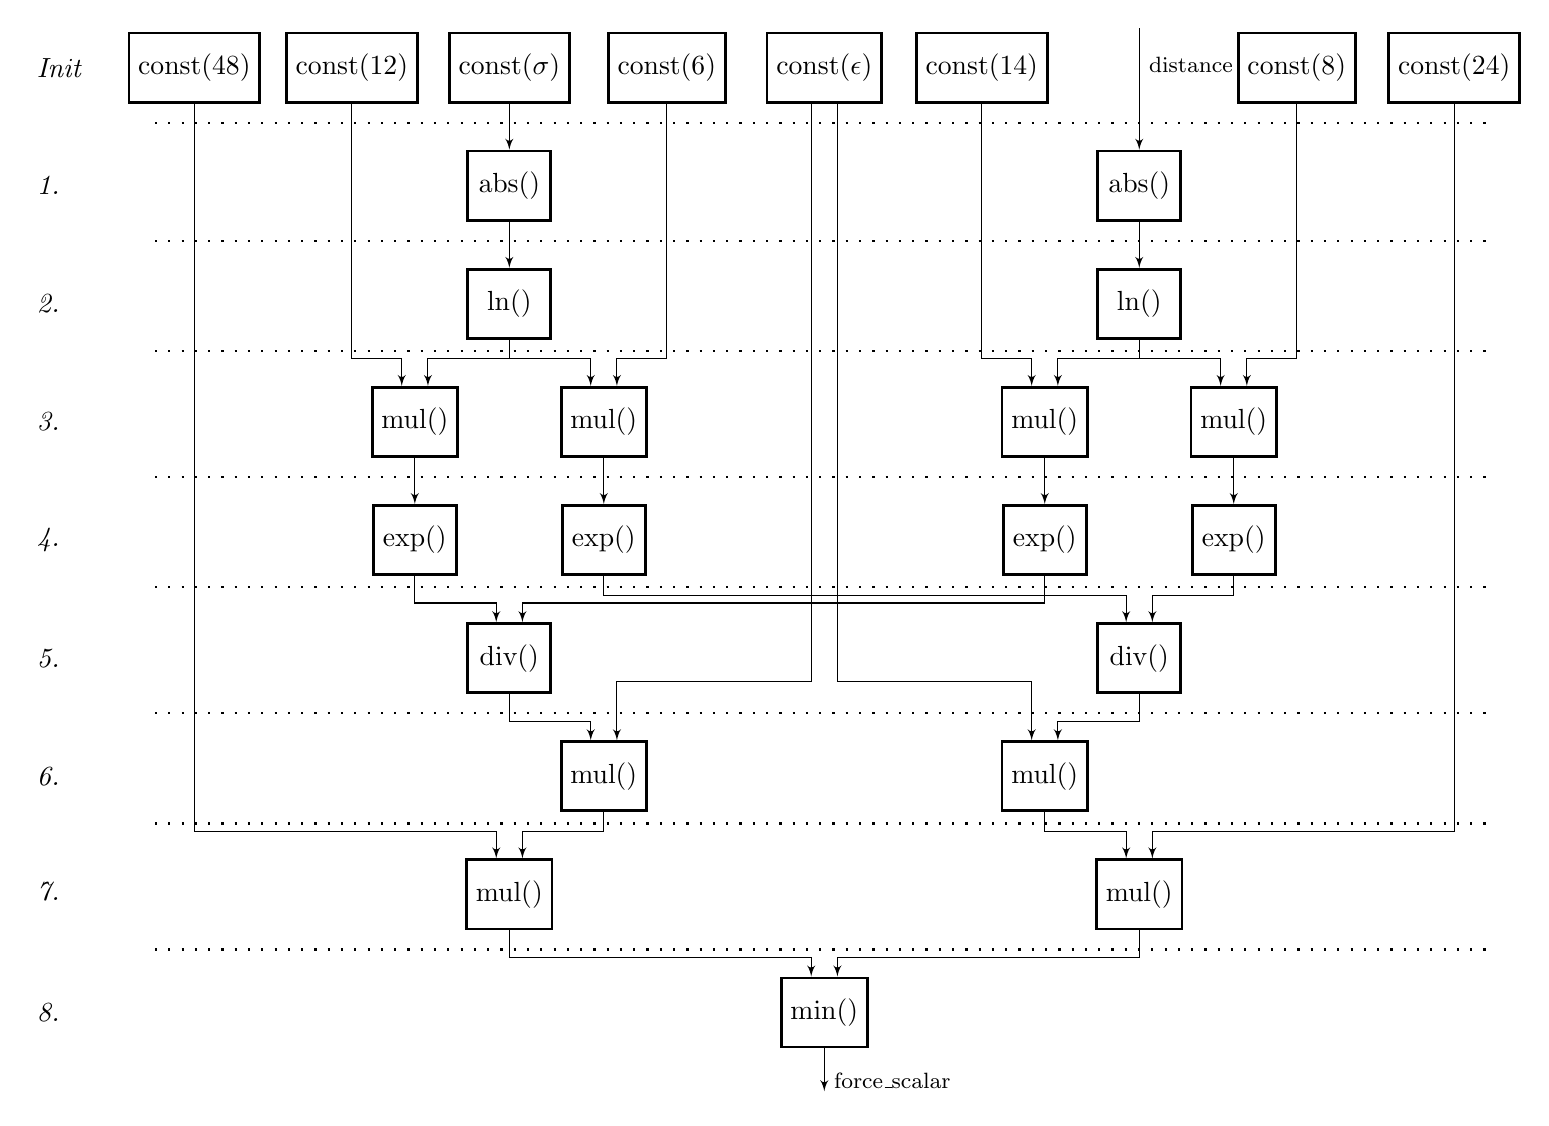
\begin{tikzpicture}

            \node[process, minimum height=2.5em] (twelve) at (-6,0) {const(12)};
            \node[process, minimum height=2.5em] (six) at (-2,0) {const(6)};
            \node[process, minimum height=2.5em] (sigma) at (-4,0) {const($\sigma$)};
            \node[process, minimum height=2.5em] (epsilon) at (0,0) {const($\epsilon$)};
            \node[process, minimum height=2.5em] (abs_sigma) at (-4,-1.5) {abs()};
            \node[process, minimum height=2.5em] (ln_sigma) at (-4,-3) {ln()};

            \node[process, minimum height=2.5em] (fourteen) at (2,0) {const(14)};
            \node[process, minimum height=2.5em] (eight) at (6,0) {const(8)};

            
            \node[process, minimum height=2.5em] (fortyeight) at (-8,0) {const(48)};
            \node[process, minimum height=2.5em] (twentyfour) at (8,0) {const(24)};


            \node[process, minimum height=2.5em] (abs_r) at (4,-1.5) {abs()};
            \node[process, minimum height=2.5em] (ln_r) at (4,-3) {ln()};
            
            
            \node[process, minimum height=2.5em] (mul_12) at (-5.2,-4.5) {mul()};
            \node[process, minimum height=2.5em] (mul_6) at (-2.8,-4.5) {mul()};

            \node[process, minimum height=2.5em] (mul_14) at (2.8,-4.5) {mul()};
            \node[process, minimum height=2.5em] (mul_8) at (5.2,-4.5) {mul()};

            \node[process, minimum height=2.5em] (exp_12) at (-5.2,-6) {exp()};
            \node[process, minimum height=2.5em] (exp_6) at (-2.8,-6) {exp()};

            \node[process, minimum height=2.5em] (exp_14) at (2.8,-6) {exp()};
            \node[process, minimum height=2.5em] (exp_8) at (5.2,-6) {exp()};
            
            \node[process, minimum height=2.5em] (div_12_14) at (-4,-7.5) {div()};
            \node[process, minimum height=2.5em] (div_6_8) at (4,-7.5) {div()};

            \node[process, minimum height=2.5em] (mul_12_14_eps) at (-2.8,-9) {mul()};
            \node[process, minimum height=2.5em] (mul_6_8_eps) at (2.8,-9) {mul()};

            \node[process, minimum height=2.5em] (mul_48) at (-4,-10.5) {mul()};
            \node[process, minimum height=2.5em] (mul_24) at (4,-10.5) {mul()};

            \node[process, minimum height=2.5em] (min) at (0,-12) {min()};
            
            \node[text width=3cm] at (-8.5,-0) {\textit{Init}};
            \draw[loosely dotted, thick] (-8.5, -0.7) -- (8.5, -0.7);
            \node[text width=3cm] at (-8.5,-1.5) {\textit{1.}};
            \draw[loosely dotted, thick] (-8.5, -2.2) -- (8.5, -2.2);
            \node[text width=3cm] at (-8.5,-3) {\textit{2.}};
            \draw[loosely dotted, thick] (-8.5, -3.6) -- (8.5, -3.6);
            \node[text width=3cm] at (-8.5,-4.5) {\textit{3.}};
            \draw[loosely dotted, thick] (-8.5, -5.2) -- (8.5, -5.2);
            \node[text width=3cm] at (-8.5,-6) {\textit{4.}};
            \draw[loosely dotted, thick] (-8.5, -6.6) -- (8.5, -6.6);
            \node[text width=3cm] at (-8.5,-7.5) {\textit{5.}};
            \draw[loosely dotted, thick] (-8.5, -8.2) -- (8.5, -8.2);
            \node[text width=3cm] at (-8.5,-9) {\textit{6.}};
            \draw[loosely dotted, thick] (-8.5, -9.6) -- (8.5, -9.6);
            \node[text width=3cm] at (-8.5,-10.5) {\textit{7.}};
            \draw[loosely dotted, thick] (-8.5, -11.2) -- (8.5, -11.2);
            \node[text width=3cm] at (-8.5,-12) {\textit{8.}};

            \path[draw, ->] (sigma.270) -- (abs_sigma.90);
            \path[draw, ->] (4,0.5) -- (abs_r.90) node [pos=0.3] {\footnotesize distance};

            \path[draw, ->] (abs_sigma.270) -- (ln_sigma.90);
            \path[draw, ->] (abs_r.270) -- (ln_r.90);


            \path[draw, ->] (twelve.270) |- (-5.5, -3.7) -| (mul_12.110);
            \path[draw, ->] (ln_sigma.270) |- (-4.5, -3.7) -| (mul_12.70);
            
            \path[draw, ->] (six.270) |- (-2, -3.7) -| (mul_6.70);
            \path[draw, ->] (ln_sigma.270) |- (-3.5, -3.7) -| (mul_6.110);

            \path[draw, ->] (fourteen.270) |- (2, -3.7) -| (mul_14.110);
            \path[draw, ->] (ln_r.270) |- (3.5, -3.7) -| (mul_14.70);
            
            \path[draw, ->] (eight.270) |- (5.5, -3.7) -| (mul_8.70);
            \path[draw, ->] (ln_r.270) |- (4.5, -3.7) -| (mul_8.110);

            \path[draw, ->] (mul_12.270) -- (exp_12.90);
            \path[draw, ->] (mul_6.270) -- (exp_6.90);

            \path[draw, ->] (mul_14.270) -- (exp_14.90);
            \path[draw, ->] (mul_8.270) -- (exp_8.90);

            \path[draw, ->] (exp_12.270) |- (-4.5, -6.8) -| (div_12_14.110);
            \path[draw, ->] (exp_14.270) |- (-3.5, -6.8) -| (div_12_14.70);

            \path[draw, ->] (exp_6.270) |- (3.5, -6.7) -| (div_6_8.110);
            \path[draw, ->] (exp_8.270) |- (4.5, -6.7) -| (div_6_8.70);

            \path[draw, ->] (div_12_14.270) |- (-3.5, -8.3) -| (mul_12_14_eps.110);
            \path[draw, ->] (epsilon.250) |- (-2.5, -7.8) -| (mul_12_14_eps.70);
            
            \path[draw, ->] (div_6_8.270) |- (3.5, -8.3) -| (mul_6_8_eps.70);
            \path[draw, ->] (epsilon.290) |- (2.5, -7.8) -| (mul_6_8_eps.110);

            \path[draw, ->] (fortyeight.270) |- (-4.5, -9.7) -| (mul_48.110);
            \path[draw, ->] (mul_12_14_eps.270) |- (-3.5, -9.7) -| (mul_48.70);

            \path[draw, ->] (twentyfour.270) |- (4.5, -9.7) -| (mul_24.70);
            \path[draw, ->] (mul_6_8_eps.270) |- (3.5, -9.7) -| (mul_24.110);

            \path[draw, ->] (mul_48.270) |- (-3.5, -11.3) -| (min.110);
            \path[draw, ->] (mul_24.270) |- (2.5, -11.3) -| (min.70);

            \path[draw, ->] (min.270) -- (0,-13) node [near end] {\footnotesize force\_scalar};

        \end{tikzpicture}
    }
    \caption{The \texttt{Force} calculation representing the entire LJ potential pipeline. Each square is a process that executes the function noted, given the input from the processes above. The horizontal lines represent each layer where the data flows between. The numbering in the left are for referencing purposes only. For each clock cycle, the data flows one layer down.}
    \label{fig:force_depth}
\end{figure*}


%--------------
% Magnitude 1.0

% Magnitude figure
\begin{figure}
    \centering
    \scalebox{0.7}{
        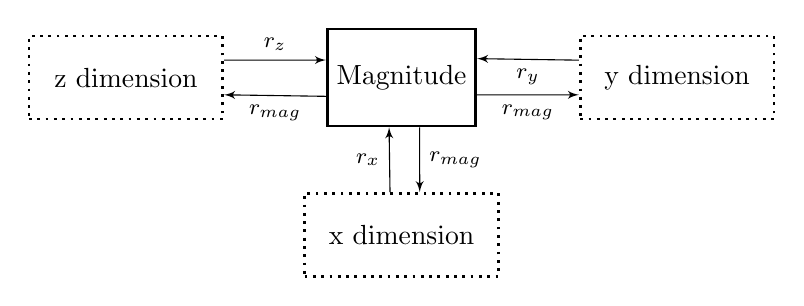
\begin{tikzpicture}
            \node[process] (magnitude) at (0,0) {Magnitude};
            \node[module, minimum height=3em, minimum width=7em] (xdim) at (0,-2) {x dimension};
            \node[module, minimum height=3em, minimum width=7em] (ydim) at (3.5,0) {y dimension};
            \node[module, minimum height=3em, minimum width=7em] (zdim) at (-3.5,0) {z dimension};

            \path[draw, ->] (xdim.105) -- (magnitude.256) node [midway] {\footnotesize $r_x$};
            \path[draw, ->] (ydim.170) -- (magnitude.14) node [midway] {\footnotesize $r_y$};
            \path[draw, ->] (zdim.10) -- (magnitude.167) node [midway] {\footnotesize $r_z$};


            \path[draw, ->] (magnitude.290) -- (xdim.67) node [midway] {\footnotesize $r_{mag}$};
            \path[draw, ->] (magnitude.347) -- (ydim.190) node [midway, below] {\footnotesize $r_{mag}$};
            \path[draw, ->] (magnitude.194) -- (zdim.350) node [midway] {\footnotesize $r_{mag}$};
        \end{tikzpicture}
    }
    \caption{The magnitude is calculated between the different dimensions. The dimensions are running in parallel and communicating with the \texttt{Magnitude} module only when the magnitude is needed in the acceleration calculations.}
    \label{fig:magnitude}
\end{figure}


% -----------------------
% MD steps

\begin{figure}
    \centering
    \scalebox{0.8}{
        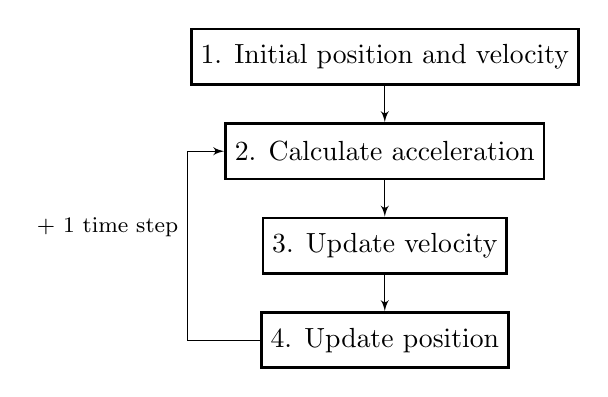
\begin{tikzpicture}
            \node[process, minimum height=2em, minimum width=7em] (init) at (0,0) {1. Initial position and velocity};
            \node[process, minimum height=2em, minimum width=7em] (acc) at (0,-1.2) {2. Calculate acceleration};
            \node[process, minimum height=2em, minimum width=7em] (vel) at (0,-2.4) {3. Update velocity};
            \node[process, minimum height=2em, minimum width=7em] (pos) at (0,-3.6) {4. Update position};

            \path[draw, ->] (init.270) -- (acc.90);
            \path[draw, ->] (acc.270) -- (vel.90);
            \path[draw, ->] (vel.270) -- (pos.90);

            \path[draw, ->] (pos.180) -| (-2.5,-3.6) |- (acc.180) node [pos=0.3] {\footnotesize + 1 time step};
        \end{tikzpicture}
    }
    \caption{The specific steps of an MD simulation. Each step requires the result of the previous step. After step 4 it loops around to step 2. Each loop is a time step.}
    \label{fig:md_steps}
\end{figure}

%--------------------------
%Pipe example

%pipe figure
\begin{figure}
    \centering
    \scalebox{0.7}{
        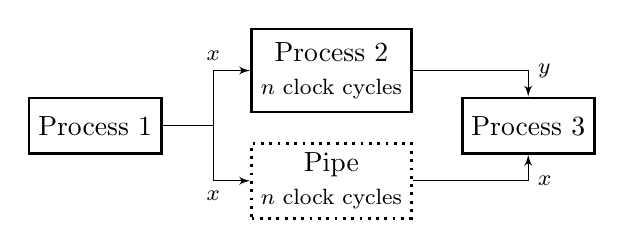
\begin{tikzpicture}
            \node[process, minimum height=2em] (proc1) at (0,0) {Process 1};
            \node[process, minimum height=2em, align=center, dotted] (pipe) at (3,-0.7) {Pipe\\ \footnotesize $n$ clock cycles};
            \node[process, minimum height=3em, align=center] (proc2) at (3,0.7) {Process 2\\ \footnotesize $n$ clock cycles};
            \node[process, minimum height=2em] (proc3) at (5.5,0) {Process 3};

            \path[draw, ->] (proc1.0) -| (1.5,0) |- (pipe.180) node [midway, below] {\footnotesize $x$};
            \path[draw, ->] (proc1.0) -| (1.5,0) |- (proc2.180) node [midway, above] {\footnotesize $x$};
            \path[draw, ->] (pipe.0) -| (proc3.270) node [midway, right] {\footnotesize $x$};
            \path[draw, ->] (proc2.0) -| (proc3.90) node [midway] {\footnotesize $y$};
        \end{tikzpicture}
    }
    \caption{An example of a pipe structure that is inserted to retain data for a certain amount of clock cycles. In the figure, the \texttt{Pipe} is a collection of $n$ pipe processes, each one taking one clock cycle.}
    \label{fig:pipe}
\end{figure}

\end{document}
